

\section{The Site Calendar}
The site calendar is used to schedule all observations and testing that is carried out on meerKAT telescope. The operator will typically follow the instructions that are scheduled on this calendar to do global sync, calibration, stowing the antennas for flights, build subarrays etc. The operator will be required to do the following as per the calendar entries:

\begin{itemize}	
\item{}	Verify that you are on AR1\_site calendar, see \textbf{Figure}~\ref{fig:calendar} below for depiction of the site calendar.

\item{} If no schedule block (SB) is assigned, then proceed to the section below.
	
	
\end{itemize}




\begin{figure}[!thb]
	\centering
	%\includegraphicsdpi{100}{}{bur1.png}     
	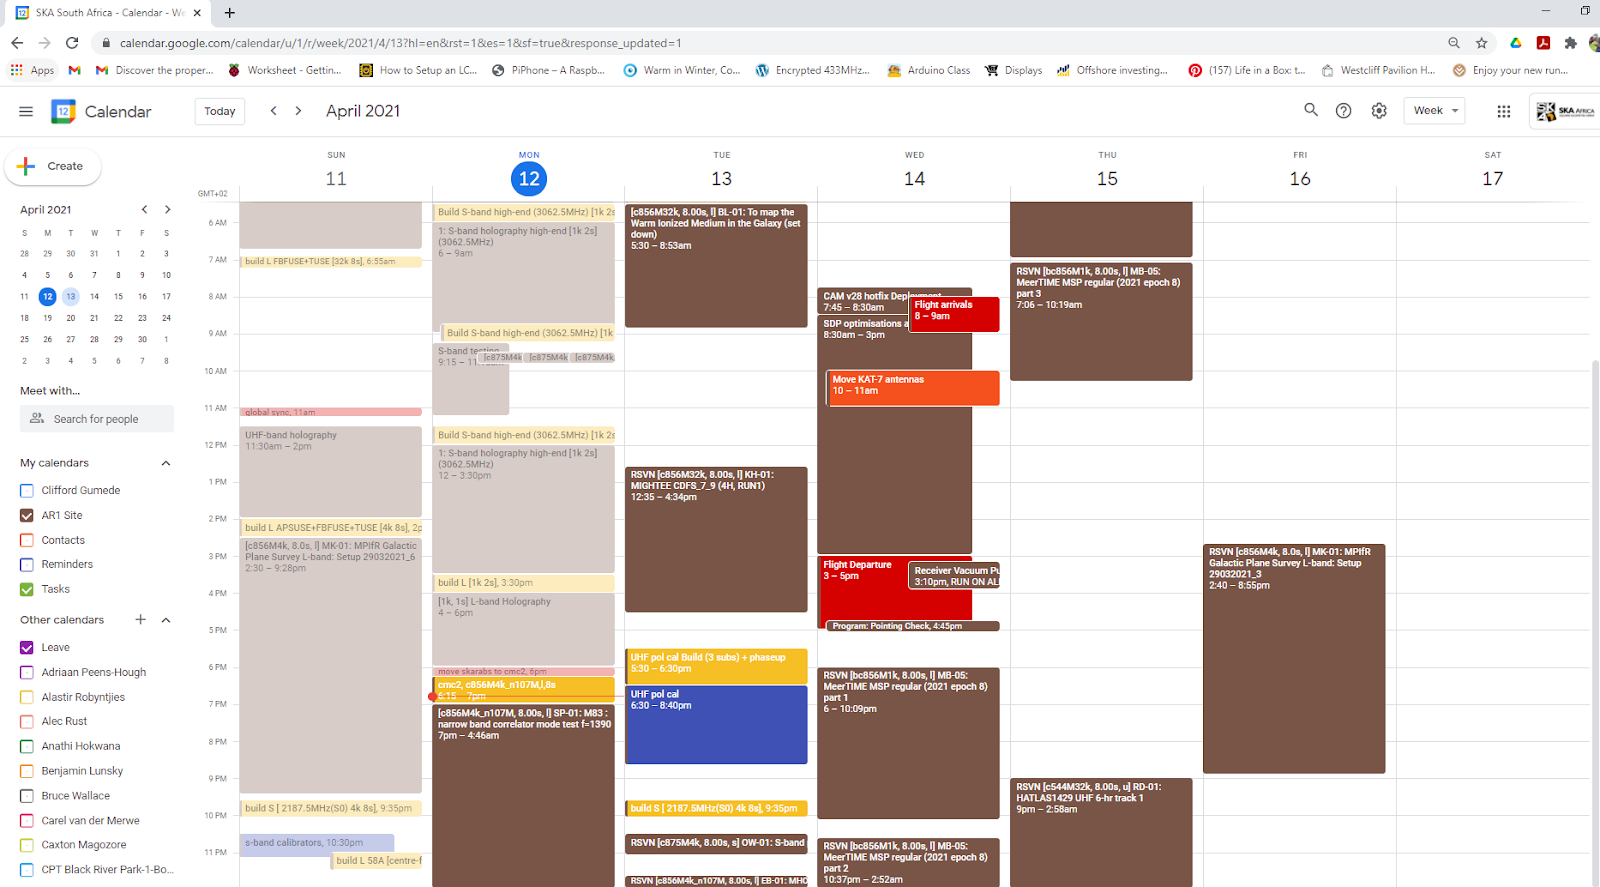
\includegraphics[scale=0.25]{Chapters/images/calendar.png}
	
	%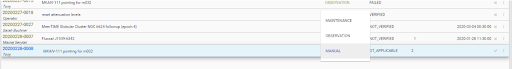
\includegraphics[resolution=100]{bur1.png}
	\caption{Google calendar for site activities}
	\label{fig:calendar}
\end{figure}
\section{ Create a New Schedule Block (SB)}
Connect to obs machine via 
\begin{lstlisting}[style=DOS]
ssh kat@obs.mkat.karoo.ac.za
ipython
Import katuilib
configure_obs()
\end{lstlisting}

	
Paste the schedule block details as shown in the image below in \textbf{Figure}~\ref{fig:image3} and run from the calendar event (observation).


\begin{figure}[!thb]
	\centering
	%\includegraphicsdpi{100}{}{bur1.png}     
	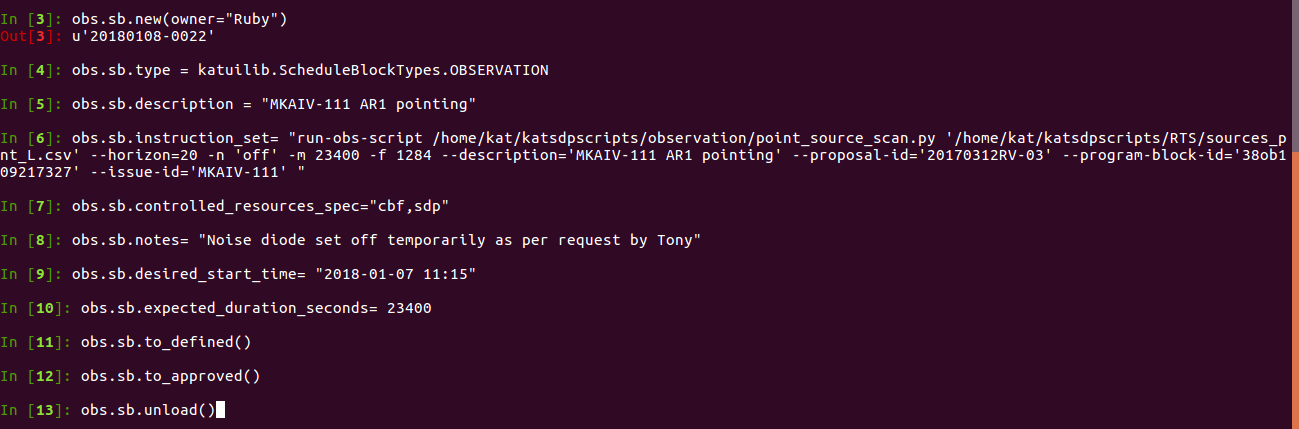
\includegraphics[scale=0.35]{Chapters/images/image3.png}
	
	%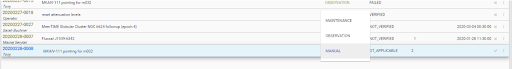
\includegraphics[resolution=100]{bur1.png}
	\caption{SB pasted on ipython sesion}
	\label{fig:image3}
\end{figure}
The commands above when ran in this ipython session will create a new SB in the GUI as shown in \textbf{Figure}~\ref{fig:image6}.

\begin{figure}[!thb]
	\centering
	%\includegraphicsdpi{100}{}{bur1.png}     
	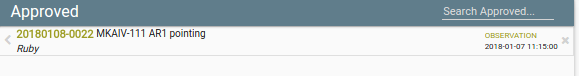
\includegraphics[scale=0.8]{Chapters/images/image6.png}
	
	%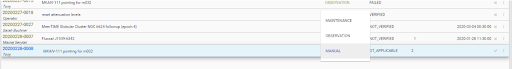
\includegraphics[resolution=100]{bur1.png}
	\caption{CAM GUI approved SB }
	\label{fig:image6}
\end{figure}

\section{Retrieve Old Schedule Blocks}
If you need to find a schedule block (SB) that is no longer found in the complete SB history in the GUI as shown in \textbf{Figure}~\ref{fig:image44} below. 

\begin{figure}[!thb]
	\centering
	%\includegraphicsdpi{100}{}{bur1.png}     
	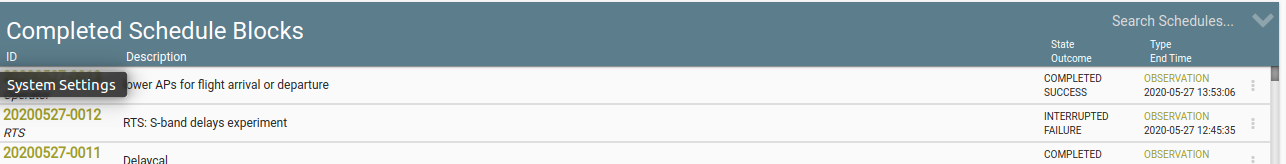
\includegraphics[scale=0.35]{Chapters/images/image44.png}
	
	%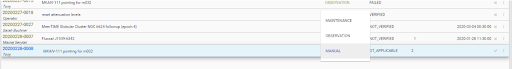
\includegraphics[resolution=100]{bur1.png}
	\caption{Completed SB search}
	\label{fig:image44}
\end{figure}

Connect to the obs machin by ssh and run the commands as shown in \textbf{Figure}~\ref{fig:image116} .
\begin{lstlisting}[style=DOS]
ssh kat@obs.mkat.karoo.kat.ac.za
\end{lstlisting}



\begin{figure}[!thb]
	\centering
	%\includegraphicsdpi{100}{}{bur1.png}     
	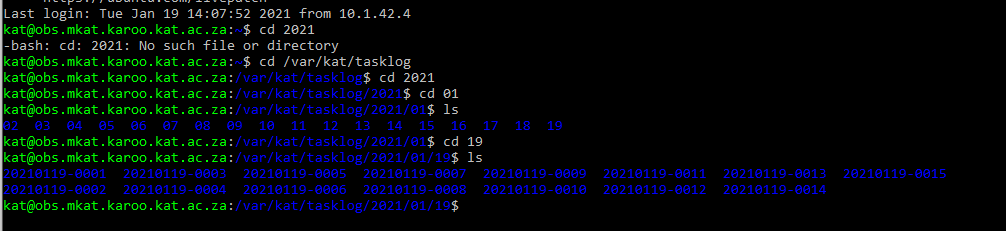
\includegraphics[scale=0.35]{Chapters/images/image116.png}
	
	%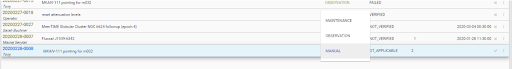
\includegraphics[resolution=100]{bur1.png}
	\caption{SB search in the obs machine}
	\label{fig:image116}
\end{figure}
Select the schedule block number that you need.
You can view the contents of the schedule block by running the following commands on the ipython session: 

\begin{lstlisting}[style=DOS]
configure_obs()
obs.sb.new_clone(sb_number'
obs.sb.load('new_sb_number' )
\end{lstlisting}


If you do not know what the SB number is but know when the observation ran, run the following commands to display list of activities as shown in \textbf{Figure}~\ref{fig:image42}
\begin{lstlisting}[style=DOS]
ssh kat@portal.mkat.karoo.kat.ac.za
cd /var/kat/log$ 
less activity.2020-05-27.log  (you can choose the date of the log you want to view)
\end{lstlisting} 



\begin{figure}[!thb]
	\centering
	%\includegraphicsdpi{100}{}{bur1.png}     
	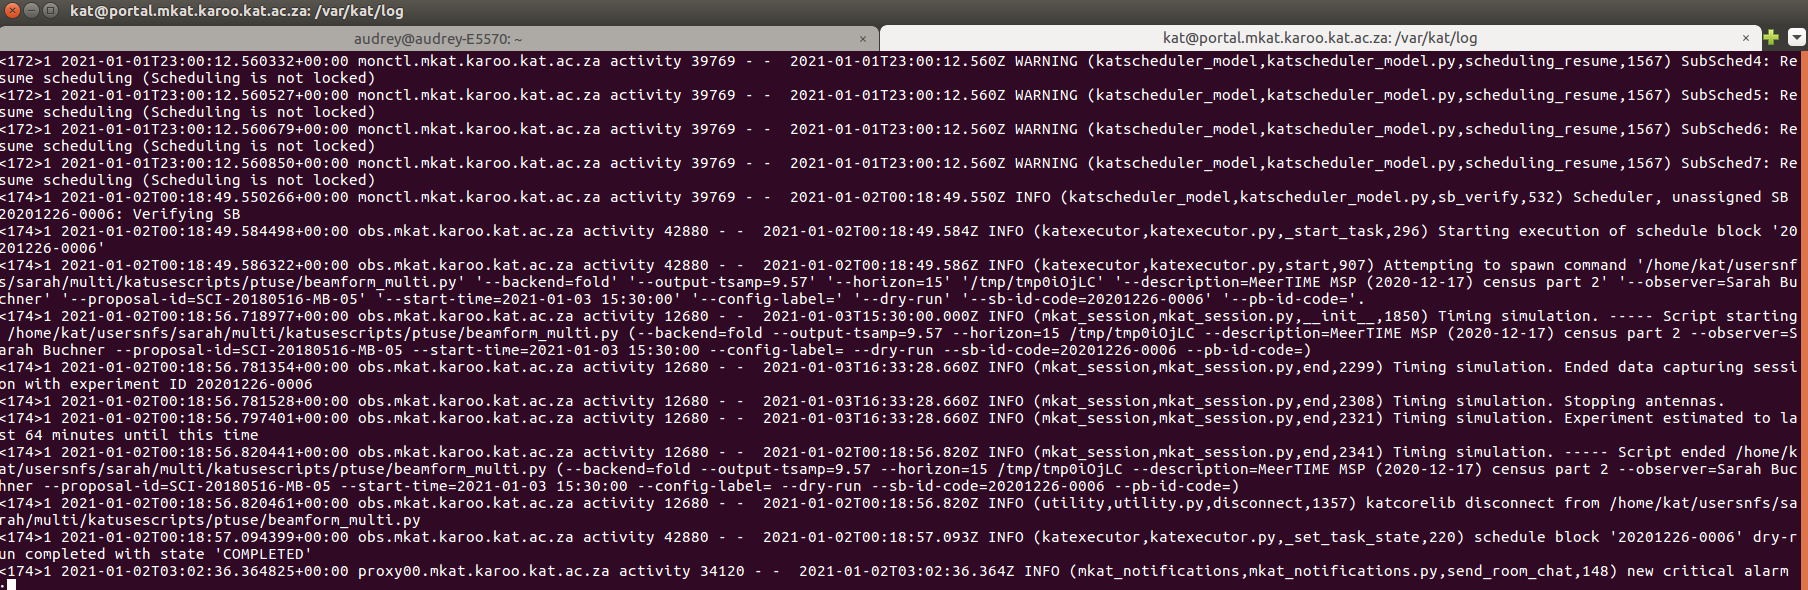
\includegraphics[scale=0.25]{Chapters/images/image42.png}
	
	%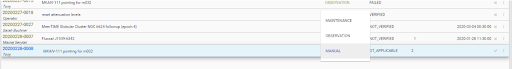
\includegraphics[resolution=100]{bur1.png}
	\caption{Open SB log file}
	\label{fig:image42}
\end{figure}
Zoom in on the screenshot to see schedule block numbers that ran/dry-ran on your chosen date.

\section{ Build a subarray (SA) suitable for the SB (observation)}
Select and load the desired resources from the free resources. These are:
Receptors (AP)
The correlator (\component{cbf\_x}) for \server{cmc1} or \component{cbf\_dev\_x} for \server{cmc2}
Science Processor (\component{sdp\_x})
Note that the Correlator and Science Processor proxy numbers denoted by \component{\_x} must match the subarray number (1 to 4) 
Select the data user product (List provided in drop down menu) 
Select desired frequency band (l,u,s or x)
Select desired dump rate (list provided in drop down menu)
If the dump rate was not specified for the SB (observation) leave the default setting as is.
Select APSUSE, FBFUSE, PTUSE and TUSE and if neededActivate the subarray. When the array is active, it will appear green in \textbf{Figure}~\ref{fig:image113}
\begin{figure}[!thb]
	\centering
	%\includegraphicsdpi{100}{}{bur1.png}     
	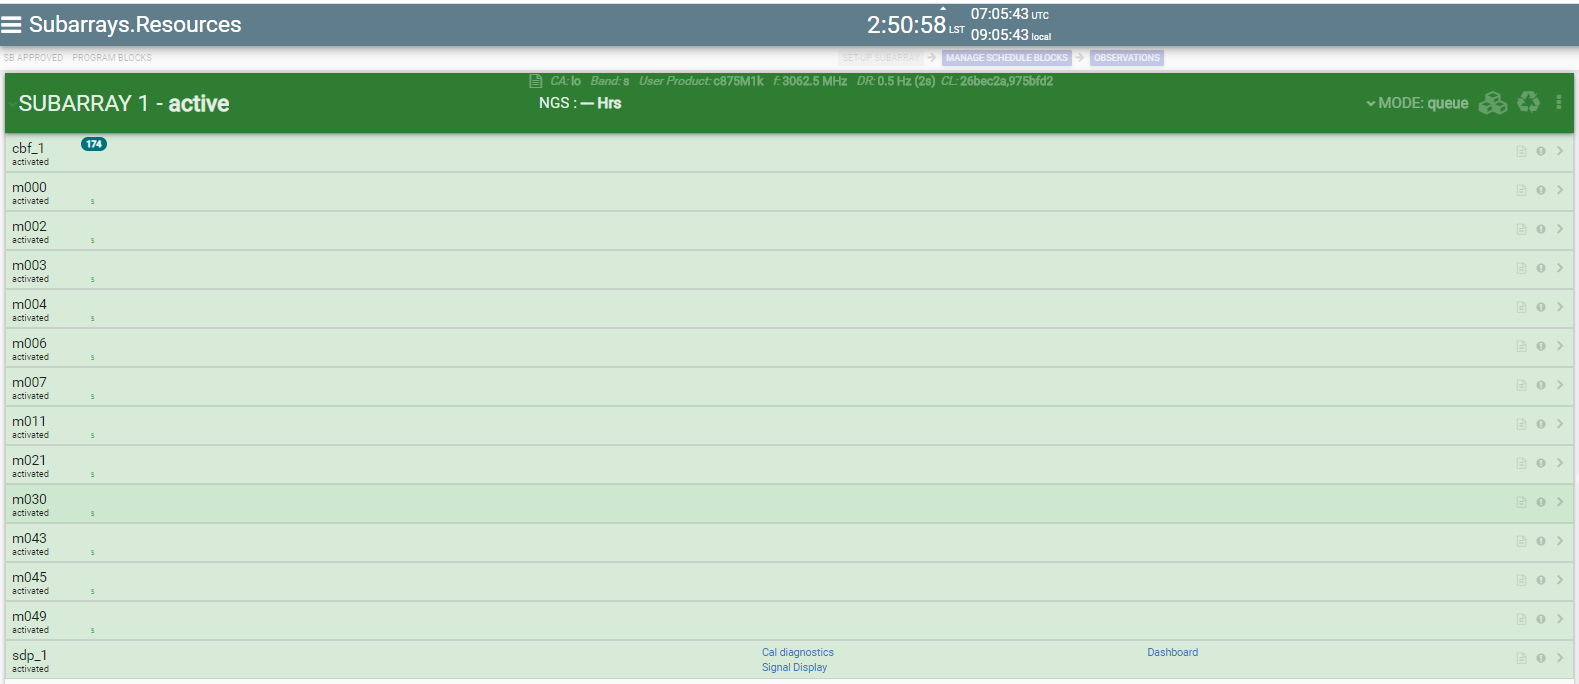
\includegraphics[scale=0.25]{Chapters/images/image113.png}
	
	%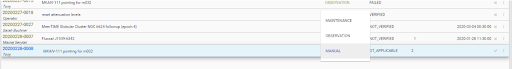
\includegraphics[resolution=100]{bur1.png}
	\caption{Active subarray with\component{cbf\_1} and \component{sdp\_1} resources}
	\label{fig:image113}
\end{figure}

Verify the SB by clicking on the far right dots of sb, see \textbf{Figure}~\ref{fig:image12}.


\begin{figure}[!thb]
	\centering
	%\includegraphicsdpi{100}{}{bur1.png}     
	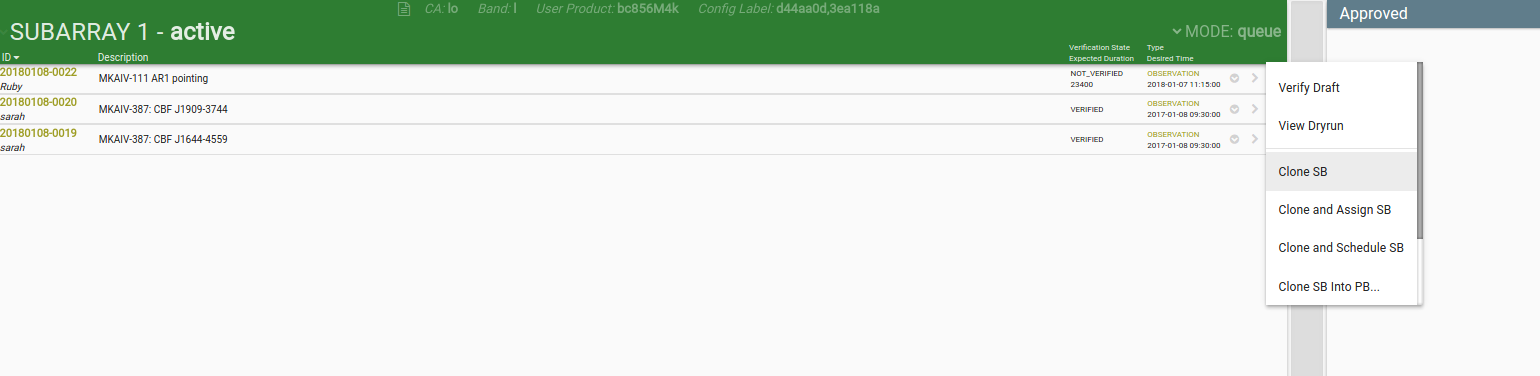
\includegraphics[scale=0.25]{Chapters/images/image12.png}
	
	%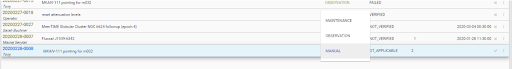
\includegraphics[resolution=100]{bur1.png}
	\caption{ Verifying a SB }
	\label{fig:image12}
\end{figure}
\begin{itemize}
\item While verifying, check the dry run,
\item run the Schedule Block 
\item Schedule the SB
\item Execute the schedule
\item Scheduler modes should be in 
\begin{itemize}
\item[$\circ$] Manual - manual control over observation start-ups
\item[$\circ$] Queue - observations will automatically run as per queue
\end{itemize}
\end{itemize}
\section{ Alternative SA building using IPython session for debugging}

\#Creating a small subarray using python session
\begin{lstlisting}[style=DOS]
f=configure_subarray('test', 1)  ## build  a subarray (this is after the subarray is activated in the GUI), 'test' is the name of subarray '1' stand for subarray 1.
f.sub.sensor.number_ants.get_value()  ## to check if the subarray is active
f.ants.req.mode("STOP")
f.ants.req.target_azel(200,15)
f.ants.req.mode("POINT")
\end{lstlisting} 


This example illustrate how to run a subarray manually using CAM commands

\section{ Converting type of SB from 'MANUAL' to 'OBSERVATION'}

There are times when instruction sets could generate schedule blocks on the GUI with the observation type as MANUAL as in  \textbf{Figure}~\ref{fig:image19} :


\begin{figure}[!thb]
	\centering
	%\includegraphicsdpi{100}{}{bur1.png}     
	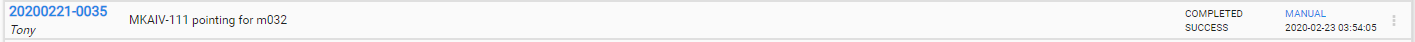
\includegraphics[scale=0.25]{Chapters/images/image19.png}
	
	%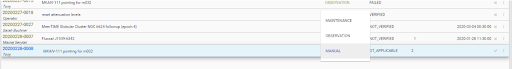
\includegraphics[resolution=100]{bur1.png}
	\caption{Manual SB}
	\label{fig:image19}
\end{figure}

If this happens, the dry run and progress log will be empty. The observation type can be changed on the GUI by following the steps below:

First assign the SB to the subarray as shown in  \textbf{Figure}~\ref{fig:image131}


\begin{figure}[!thb]
	\centering
	%\includegraphicsdpi{100}{}{bur1.png}     
	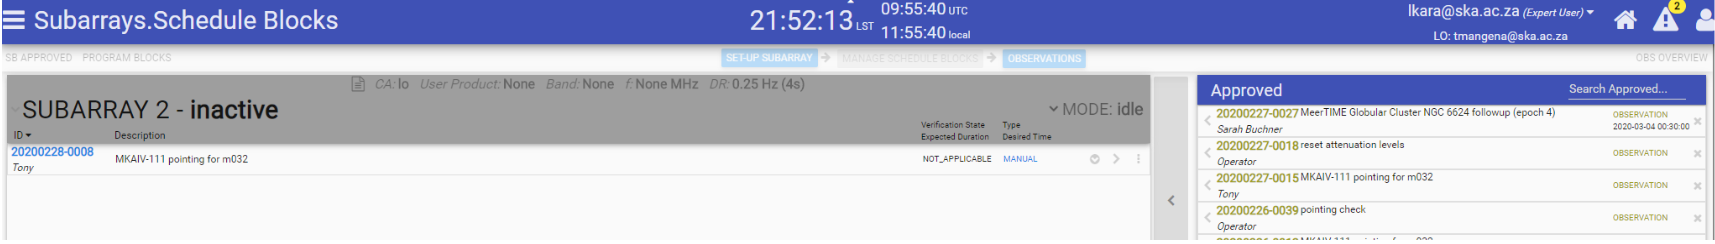
\includegraphics[scale=0.25]{Chapters/images/image131.png}
	
	%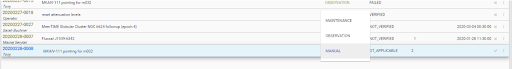
\includegraphics[resolution=100]{bur1.png}
	\caption{A SB assigned  to a subarray\_2}
	\label{fig:image131}
\end{figure}

Click on ‘SB APPROVED’, see  \textbf{Figure}~\ref{fig:image119}


\begin{figure}[!thb]
	\centering
	%\includegraphicsdpi{100}{}{bur1.png}     
	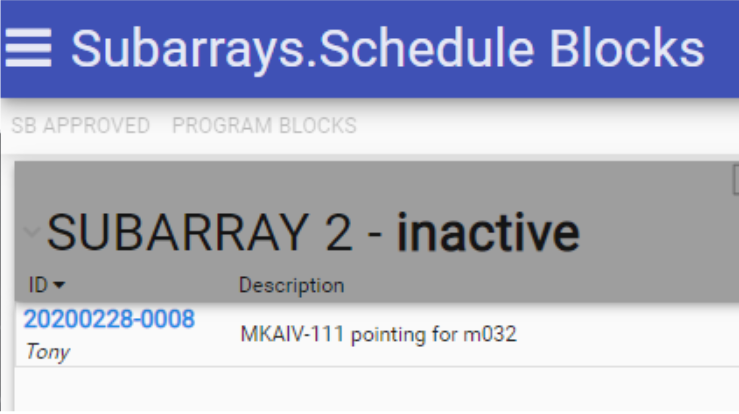
\includegraphics[scale=0.25]{Chapters/images/image119.png}
	 
	%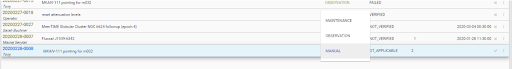
\includegraphics[resolution=100]{bur1.png}
	\caption{Approved SB}
	\label{fig:image119}
\end{figure}

Choose ‘Edit’ as shown in \textbf{Figure}~\ref{fig:image31}
\begin{figure}[H]
	\centering
	%\includegraphicsdpi{100}{}{bur1.png}     
	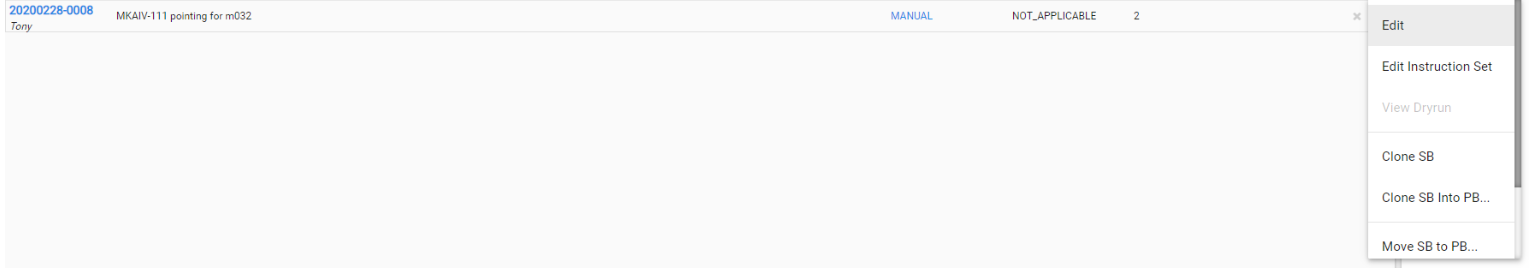
\includegraphics[scale=0.25]{Chapters/images/image31.png}
	
	%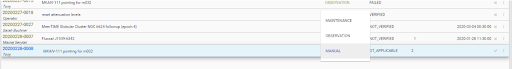
\includegraphics[resolution=100]{bur1.png}
	\caption{Edit the approved SB}
	\label{fig:image31}
\end{figure}


Choose ‘OBSERVATION’ in the drop-down menu under ‘TYPE’

\begin{figure}[H]
	\centering
	%\includegraphicsdpi{100}{}{bur1.png}     
	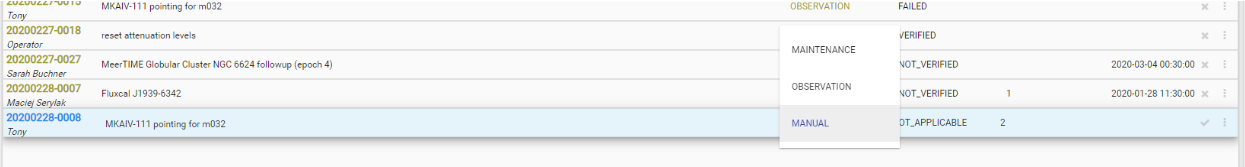
\includegraphics[scale=0.37]{Chapters/images/image53.png}
	
	%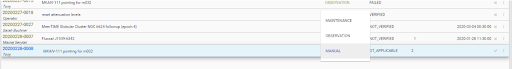
\includegraphics[resolution=100]{bur1.png}
	\caption{Save SB as observation type}
	\label{fig:image53}
\end{figure}


Save that option by clicking on the tick



\begin{figure}[!thb]
	\centering
	%\includegraphicsdpi{100}{}{bur1.png}     
	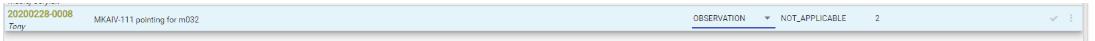
\includegraphics[scale=0.4]{Chapters/images/ManualSB.png}
	
	%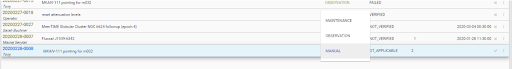
\includegraphics[resolution=100]{bur1.png}
	\caption{Save the edited SB }
	\label{fig:ManualSB}
\end{figure}

If you verify the SB this time, it should give you a dry run.

\section{Reset Attenuations}

This script can be run immediately after building an array when antennas have been out for maintenance or when changing between bands.

The power level into the digitiser (\sensor{rfcu.hpol.rf.power.in}) cannot be adjusted as this is a measure of the signal power produced by the receiver. Gain adjustment inside the receiver is not possible. If this power level is in error, operations should investigate the health of the receiver.
Operations can, and should, however adjust the power level that enters the ADC (\sensor{adc.hpol.rf.power.in}). If this sensor is in ERROR, operations should firstly verify the state of the RF power into the digitiser (\sensor{rfcu.hpol.rf.power.in}) to ensure that it is not in ERROR. If not the gain of the digitiser should be determined to ensure that it is within limits. Once it has been verified that the gain is within limits, the digitiser attenuation must be decreased until the power level into the ADC is within limits. There is no need for all the attenuators to be set to the same value. The reason for the attenuators is to adjust each receptor values individually. I therefore expect to see variations in attenuation across the array.

The second thing to remember is that the digitiser has a lot of dynamic range which means that there is very little chance of any saturation happening in the digitiser. You should therefore not unnecessarily add attenuation. It would be better to reduce attenuation (more gain) than add attenuation.

Attenuation levels should always be set to appropriate levels depending on the target brightness.  For very bright sources, attenuation levels are set at 31.  For most of our observations attenuation levels are set 6 for L-band.

Source:
\begin{lstlisting}[style=DOS]
kat@obs.mkat.karoo.kat.ac.za:~$ less STANDARD_SCHEDULE_BLOCKS.TXT 
\end{lstlisting}


In the obs machine, you must login ipython session and run: 
\begin{lstlisting}[style=DOS]
configure_obs()
obs.sb.new(owner='SeanPassmoor')
obs.sb.type=katuilib.ScheduleBlockTypes.OBSERVATION
obs.sb.description='Reset  attenuation levels'
obs.sb.antenna_spec='available'
obs.sb.instruction_set="run-obs-script /home/kat/katsdpscripts/utility/set_attenuation.py /home/kat/katsdpscripts/utility/AttenuationValues.csv"
obs.sb.to_defined()
obs.sb.to_approved()
\end{lstlisting}



You may consult with the AOD if the power levels do not look levelled, or look suspicious. There is a script below that you can run to refine attenuations found in the same folder above.

On the terminal, run:
\begin{lstlisting}[style=DOS]
ssh kat@obs.mkat.karoo.kat.ac.za
ipython
\end{lstlisting}
and paste the following SB:

\begin{lstlisting}[style=DOS]
configure_obs()
obs.sb.new(owner="SeanPassmoor") 
obs.sb.type = katuilib.ScheduleBlockTypes.OBSERVATION
obs.sb.description = "Refine Attenuation" 
obs.sb.antenna_spec="available"
obs.sb.instruction_set= "run-obs-script /home/kat/katsdpscripts/utility/refine_attenuation.py"
obs.sb.proposal_id='CAL-Attenuate'
obs.sb.to_defined()
obs.sb.to_approved()
obs.sb.unload()

\end{lstlisting}

\section{ Setting digitiser attenuation via ipython session}
On the \server{obs} machine/server. Configure a cam object:
 \begin{lstlisting}[style=DOS]
 ssh kat@obs.mkat.karoo.kat.ac.za
 ipython
 import katuilib
 configure_cam('camcam','all')
 \end{lstlisting}


Check attenuation:
\begin{lstlisting}[style=DOS]
cam.print_sensors('attenuation')

\end{lstlisting}

The steps below must be done before building a subarray but it is not advisable to set attenuations manually as there is a script that  was developed that has automated this process. These steps below can be used for test purposes only.


\subsection{ To attenuate all digitiser}
\begin{lstlisting}[style=DOS]
cam.ants.req.dig_attenuation('h',6)  
cam.ants.req.dig_attenuation('v',6)
\end{lstlisting}

This will apply attenuation of 6 to both vertical (v) and horizontal(h) polarisations of all antennas. This must not be done under any circumstances unless debugging the system. 
\subsection {To attenuate a single digitiser}
\begin{lstlisting}[style=DOS]
cam.m0xx.req.dig_attenuation('h',6)  
cam.m0xx.req.dig_attenuation('v',6) 
\end{lstlisting}
 
\section{ Delay Calibration and Phase-ups}
This is done to ensure that the signal has a phase difference of zero. Solutions close to zero are acceptable but monitor the waterfall plot as indicated below if unsure. To find a procedure on how access signal displays and plot waterfall displays go, go to the section called “Monitor an active observation” in this manual.

Risk
Incorrect delay solutions or out of phase signal data on some baselines

Source:
\begin{lstlisting}[style=DOS]
kat@obs.mkat.karoo.kat.ac.za:~$ less STANDARD_SCHEDULE_BLOCKS.TXT
\end{lstlisting}

 

\file{calibrate\_delays} and \file{bf\_phaseup} have been updated to use the new 'default' gain feature in CBF. It is no longer necessary to specify \option{fft-shift} and \option{f-engine-gain} options in the instruction set. 
Run a delay cal immediately after every new subarray build
Monitor the progress output of the script and waterfall plot of all baselines

\subsection{Delay calibration SB}
The following SB is the Standard delay calibration. This can be run for 1K, 4K, 32K and in UHF-band and L-band.
\begin{lstlisting}[style=DOS]
configure_obs()
obs.sb.new(owner='Operator')
obs.sb.type=katuilib.ScheduleBlockTypes.OBSERVATION
obs.sb.controlled_resources_spec='cbf,sdp'
obs.sb.description='Delaycal'
obs.sb.instruction_set="run-obs-script /home/kat/katsdpscripts/observation/calibrate_delays.py '/home/kat/katsdpcatalogues/three_calib.csv' -t 128"
obs.sb.proposal_id='CAL-20200106-OP-02'
obs.sb.notes='Delay calibration.'
obs.sb.to_defined()
obs.sb.to_approved()
obs.sb.unload()
\end{lstlisting}


\subsection {Phaseup calibration SB}
The following SB is the Standard phase up with bandpass flattening. This can be run for 1K, 4K, 32K and in UHF-band and L-band.
\begin{lstlisting}[style=DOS]
configure_obs()
obs.sb.new(owner='Operator')
obs.sb.type=katuilib.ScheduleBlockTypes.OBSERVATION
obs.sb.controlled_resources_spec='cbf,sdp'
obs.sb.description='Phase up with flatten bandpass'
obs.sb.instruction_set="run-obs-script /home/kat/katsdpscripts/observation/bf_phaseup.py '/home/kat/katsdpcatalogues/three_calib.csv' -t 256 --flatten-bandpass"
obs.sb.proposal_id='CAL-20200106-OP-03'
obs.sb.notes='Phase up with bandpass flattening.'
obs.sb.to_defined()
obs.sb.to_approved()
obs.sb.unload()
\end{lstlisting}

 
\textbf{Accepted waterfall plots} - in  \textbf{Figure}~\ref{fig:image1}, looking from the top of each y-axis baseline block (time)
Green colour means there is no phase difference - this is good. Other colours are acceptable too. These are minor differences.


\begin{figure}[!thb]
	\centering
	%\includegraphicsdpi{100}{}{bur1.png}     
	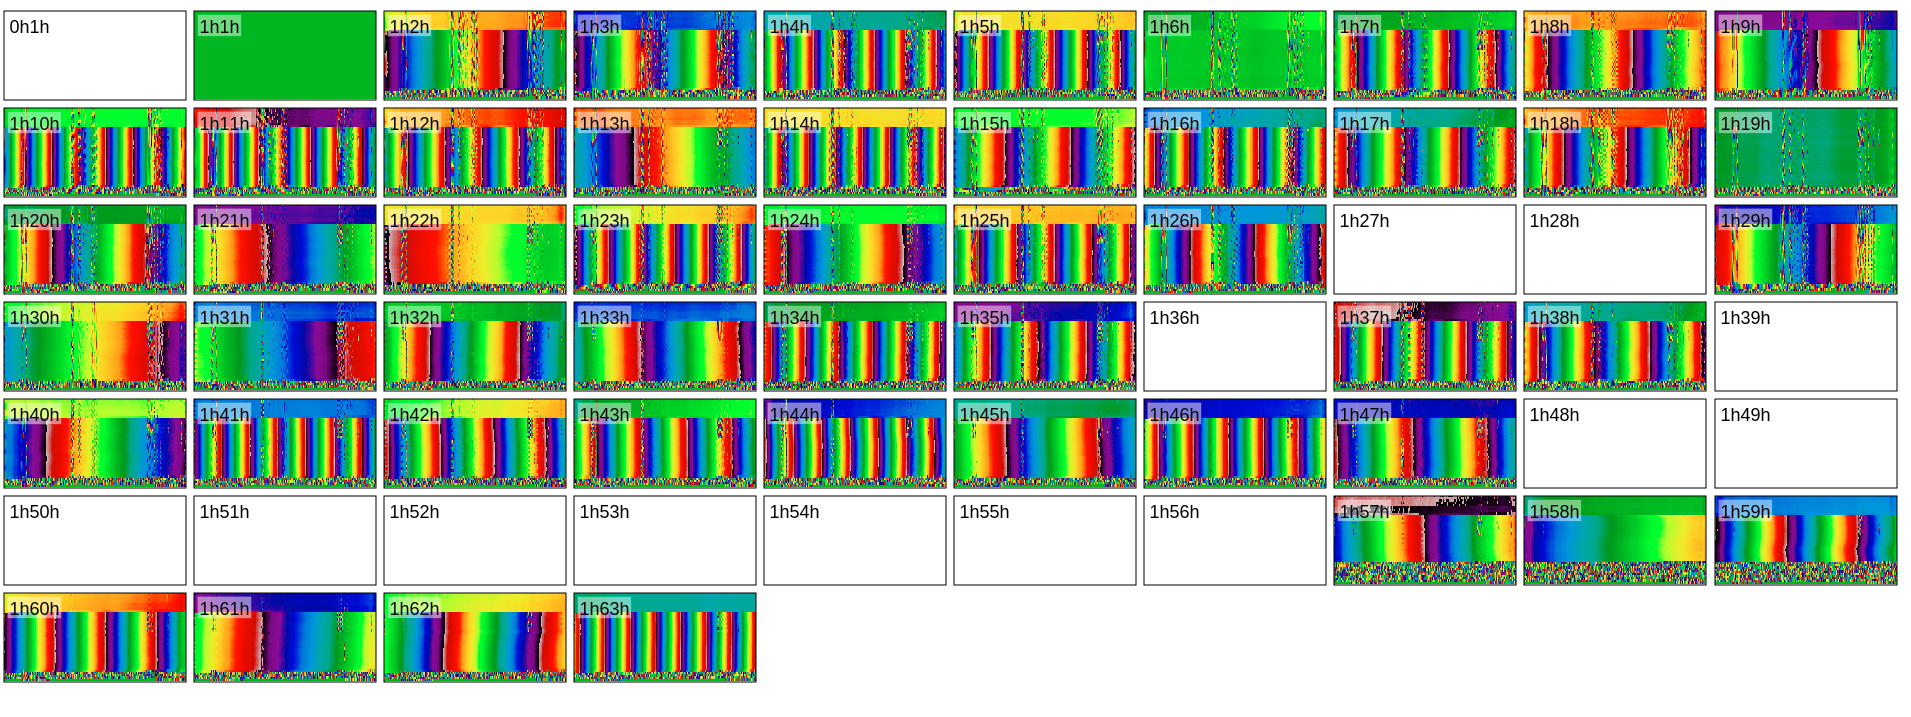
\includegraphics[scale=0.37]{Chapters/images/image1.png}
	
	%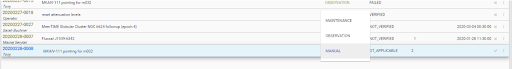
\includegraphics[resolution=100]{bur1.png}
	\caption{Acceptable waterfall plot}
	\label{fig:image1}
\end{figure}

\begin{itemize}
	\item {} For \textbf{all observation types},  noisy output/incoherent signal output is not acceptable, mark that antenna faulty.
	

	\item {} For \textbf{imaging observations}, phase wrapping can be corrected by the Astronomer, do not mark that antenna faulty.
	\item {} For \textbf{Holography and Pulsar observations}, any large delay solution values, mark the antenna faulty.
	
\end{itemize}




\subsection{  Delay Cal Script Fails:}

Delay solutions not found:\\
\option{\textcolor{red}{
2020-08-31 16:32:39.386Z WARNING   - m063h:      0.000 ns, delay fit failed (all its data probably flagged)\\
2020-08-31 16:32:39.387Z WARNING   - m063v:      0.000 ns, delay fit failed (all its data probably flagged)}
}\\

\begin{itemize}
\item{} Check \server{kat@portal.mkat.karoo.kat.ac.za:/var/kat/log}\$
(specific antenna log) - to see if the antenna misbehaved during the delay cal. e.g ap failures/proxy not in STOP when it should be.

\item{} Or check \server{kat@portal.mkat.karoo.kat.ac.za:/var/kat/log}\$ for\file{kat.cbfmon\_1} logs to see around that time that the array was built if there were any HMC or sync errors or any other cbf error regarding a F-host/X-host connected to that failed antenna.
\item{} Check cal pipeline logs via mesos in the GUI  

	
\end{itemize}

 

\section{ What could go wrong?}
\subsection{ Failed to select band while building array}
\begin{itemize}
\item{} One or more receptors failed to select observing band. The following error can be seen when building an array from the subarray logs:\\ \option{ 'select\_band\#012 raise faults. SelectBandError(failed)\#012SelectBandError: Failed to select\_band on receptors [m0xx]'} 
\item{} Wait for the building process to end, then press the retry button on the GUI.
\item{} If the above step fails, check the \sensor{'indexer raw position'} sensor in sensor list (see \textbf{Figure}~\ref{fig:image72}) for that receptor (e.g L band $=$ 40\unit{deg})

\begin{figure}[!thb]
	\centering
	%\includegraphicsdpi{100}{}{bur1.png}     
	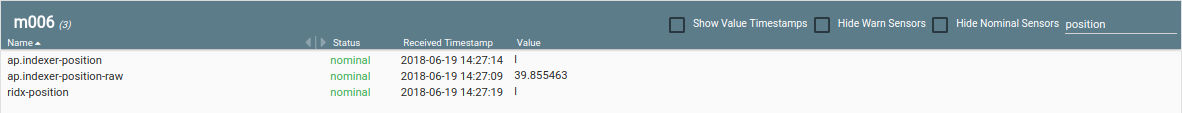
\includegraphics[scale=0.37]{Chapters/images/image72.png}
	
	%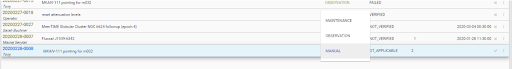
\includegraphics[resolution=100]{bur1.png}
	\caption{CAM GUI sensor list to check indexer position}
	\label{fig:image72}
\end{figure}

If not on band, ssh into the obs machine as previously done.
\begin{lstlisting}[style=DOS]
ipython
import katuilib
configure_cam('camcam', 'all')
cam.m0xx.req.mode('STOP')
cam.m0xx.req.select_band('l', timeout=60) or 'u' for UHF  
cam.m0xx.req.ap_set_indexer_position('l') or 'u' for UHF
\end{lstlisting}


\item{} If the above step fails, check if the digitiser for the band in use is marked ready as shown in \textbf{Figure}~\ref{fig:image9}. If not refer to ‘mark digitiser ready’ section on this document, or follow the steps on the  Mark Digitiser Absent and/or Ready procedure.

\begin{figure}[!thb]
	\centering
	%\includegraphicsdpi{100}{}{bur1.png}     
	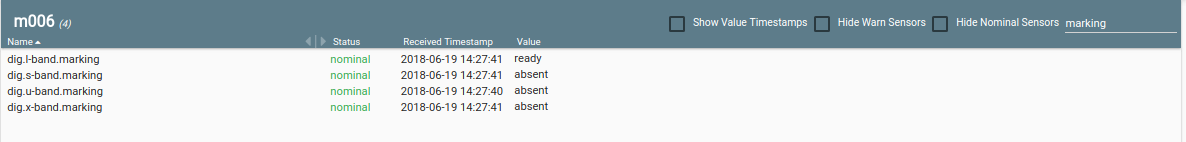
\includegraphics[scale=0.37]{Chapters/images/image9.png}
	
	%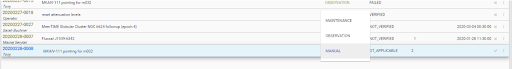
\includegraphics[resolution=100]{bur1.png}
	\caption{CAM GUI sensor list to check digitiser marking}
	\label{fig:image9}
\end{figure}
\item{} If unresolved, check if the digitiser serial number is the right one. To do this refer to the ‘Updating config for a replaced digitiser’ section on the document or follow the Checking digitiser serial numbers procedure. Should the wrong digitiser be marked ready or the issue remain unresolved contact CAM Support.
\end{itemize}

\subsection{ Multiple F-hosts in error after subarray build}

\begin{itemize}
	\item {}To identify the disabled f-hosts
	
	\begin{itemize}
		\item[$\circ$] Once the cbf is activated check the cbfmon plot in the GUI
		\item[$\circ$] The antennas appears as a green (zero) blocks in waterfall plot
		\item[$\circ$] You will see the signal for the affected antenna drop in the time series plot
		\item[$\circ$] You will also notice no ingest data on the signal display as shown in \textbf{Figure}~\ref{fig:image20}.   Type \option{flagcount} to display the figure below.
		
		
	\end{itemize}



 

\begin{figure}[!thb]
	\centering
	%\includegraphicsdpi{100}{}{bur1.png}     
	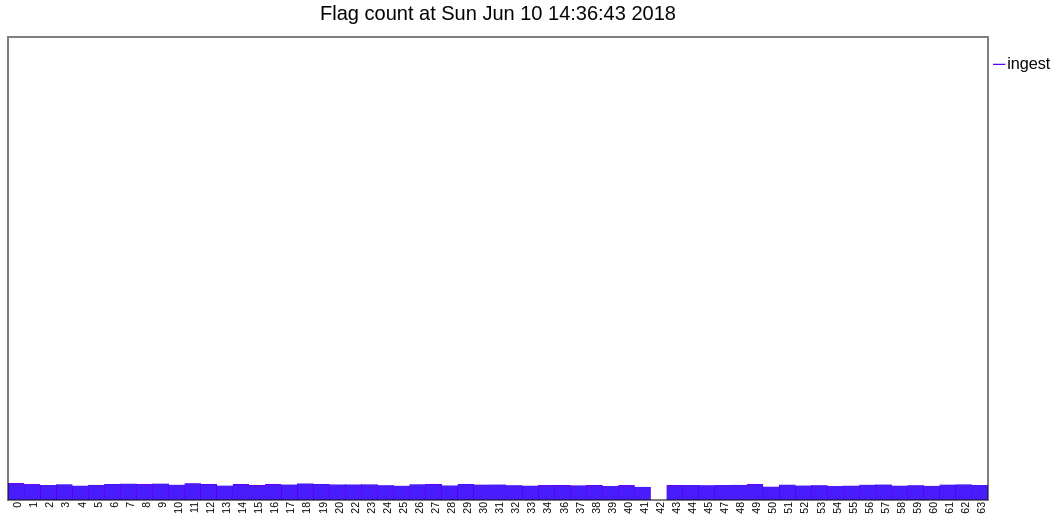
\includegraphics[scale=0.4]{Chapters/images/image20.png}
	
	%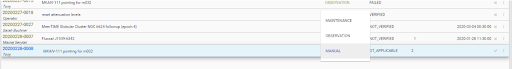
\includegraphics[resolution=100]{bur1.png}
	\caption{SDP flag count plot with one F-host disabled}
	\label{fig:image20}
\end{figure}

\item{} CBF should automatically disable a faulty F-HOST.
\item{} To verify cbf health, go to:\\ \url{http://cbf-nuc2.cpt.kat.ac.za/cmc1/array_1.wide}

\begin{figure}[!thb]
	\centering
	%\includegraphicsdpi{100}{}{bur1.png}     
	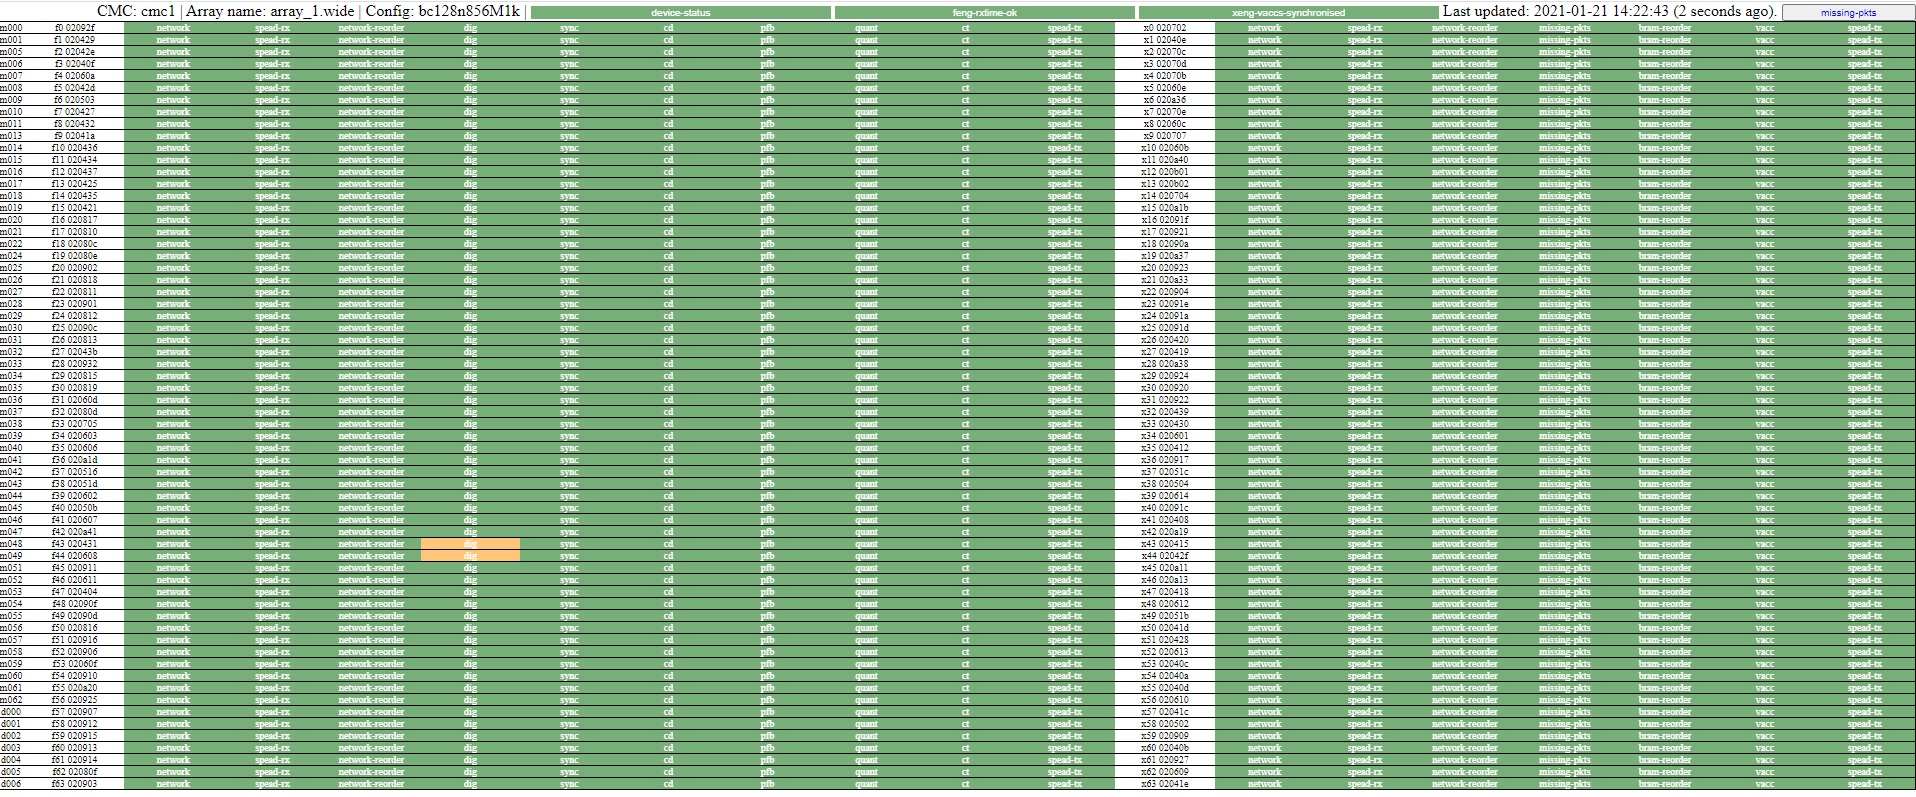
\includegraphics[scale=0.22]{Chapters/images/image40.png}
	
	%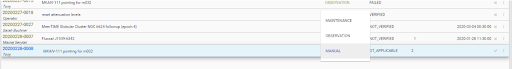
\includegraphics[resolution=100]{bur1.png}
	\caption{CBF health dashboard}
	\label{fig:image40}
\end{figure}

\item{} You can also check the sensors by looking at the CBFMON on the sensor list (hide nominal - this takes a while to load)
\item{} If multiple F-hosts are in error, break the array and build a new one [Remember to double check over a few minutes to see if the errors do not disappear by themselves.]
\item{} The other option is to check the health of CBF via the CAM GUI as shown in \textbf{Figure}~\ref{fig:image40} and \textbf{Figure}~\ref{fig:image91}

\end{itemize}


\begin{figure}[!thb]
	\centering
	%\includegraphicsdpi{100}{}{bur1.png}     
	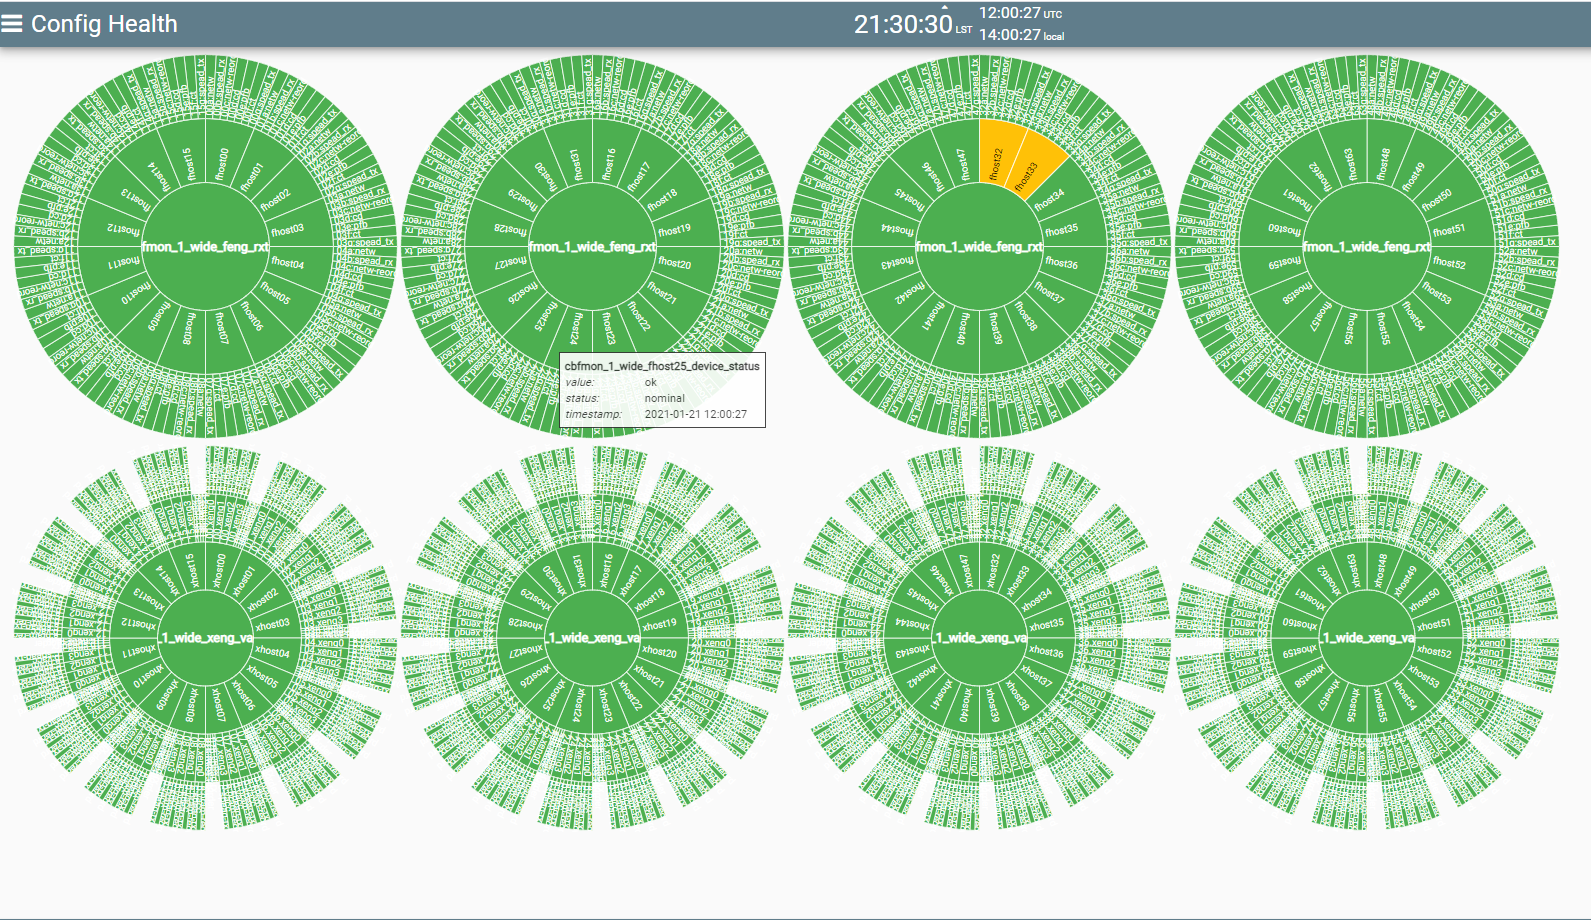
\includegraphics[scale=0.26]{Chapters/images/image91.png}
	
	%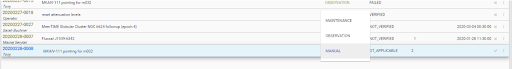
\includegraphics[resolution=100]{bur1.png}
	\caption{CBF health pie charts}
	\label{fig:image91}
\end{figure}

\subsection{ Marking SKARAB Board on Standby}	
If these f-host errors are mapped to one particular bad skarab board call cbf to disable the board.
In obs machine type the following commands to check on CMC2:
\begin{lstlisting}[style=DOS]
kcpcmd -t 30 -s 10.103.254.3:7147 array-list
kcpcmd -t 30 -s 10.103.254.3:7147 resource-list|grep "up$" | wc -l 
kcpcmd -t 10 -s 10.103.254.3:7147 resource-mark skarab020408-01 standby 
\end{lstlisting}

\subsection{ No Descriptor Errors} 
\begin{itemize}
\item{} After a subarray is built run an observation to check that descriptors are being received.
\item{} It is a good idea to run a delay cal with a long “tail” \option{--verify-duration=300}, this will return to the source for 300s after the delays are found
\end{itemize}
\subsection{ Diagnostics}
\begin{itemize}
	\item{} When running the observation it is useful to have two signals displays (windows) open
	\begin{itemize}
		\item[$\circ$] Grafana
		  \item[$\circ$]    Go to the GUI, sensor list and select sdp\_1 , Monitor descriptors in sensor list (search 'desc')
		  \item[$\circ$] The no descriptor count should not be rising
		    
		  \item[$\circ$] There are four ingest nodes - each has 1/4 of the band   
		
	\end{itemize}
	


\item{} Example of “\textbf{no descriptor}” error
	\begin{itemize}
	\item[$\circ$] No descriptor block shows orange
\item[$\circ$] Part of the band is missing, see \textbf{Figure}~\ref{fig:image79} and \textbf{Figure}~\ref{fig:image65}.
\item[$\circ$] The no descriptor heap counts keeps rising as shown in \textbf{Figure}~\ref{fig:image37}
\end{itemize}
\end{itemize}



\begin{figure}[!thb]
	\centering
	%\includegraphicsdpi{100}{}{bur1.png}     
	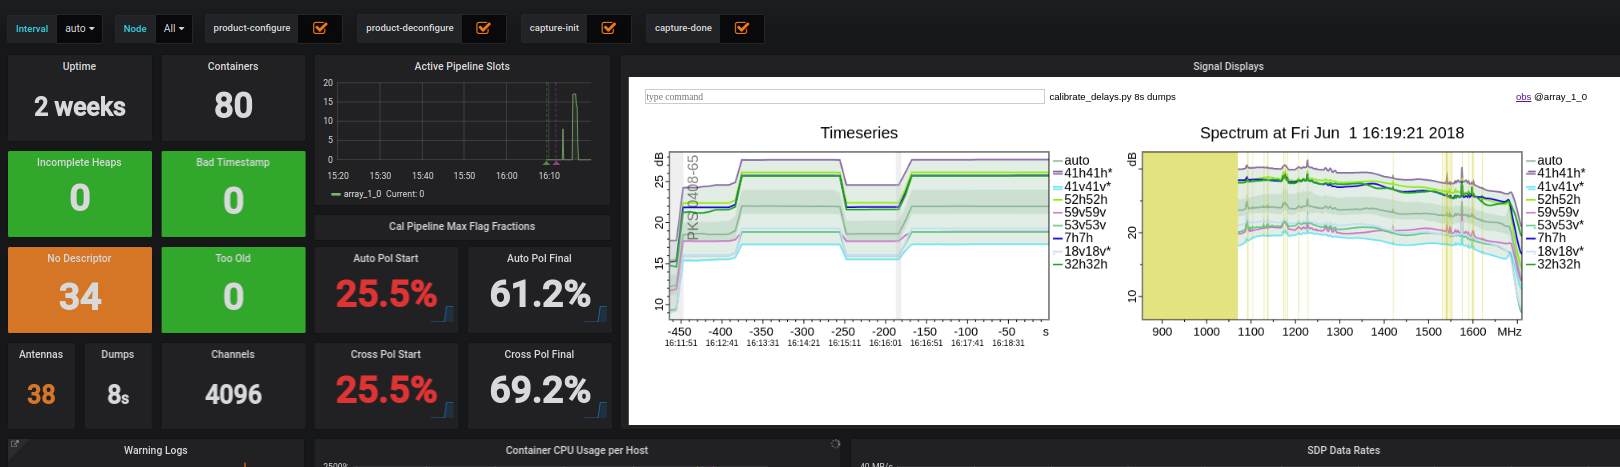
\includegraphics[scale=0.2]{Chapters/images/image79.png}
	
	%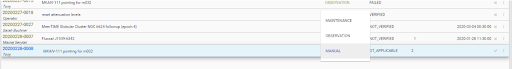
\includegraphics[resolution=100]{bur1.png}
	\caption{SDP "no descriptors" error on Grafana}
	\label{fig:image79}
\end{figure}

\begin{figure}[H]
	\centering
	%\includegraphicsdpi{100}{}{bur1.png}     
	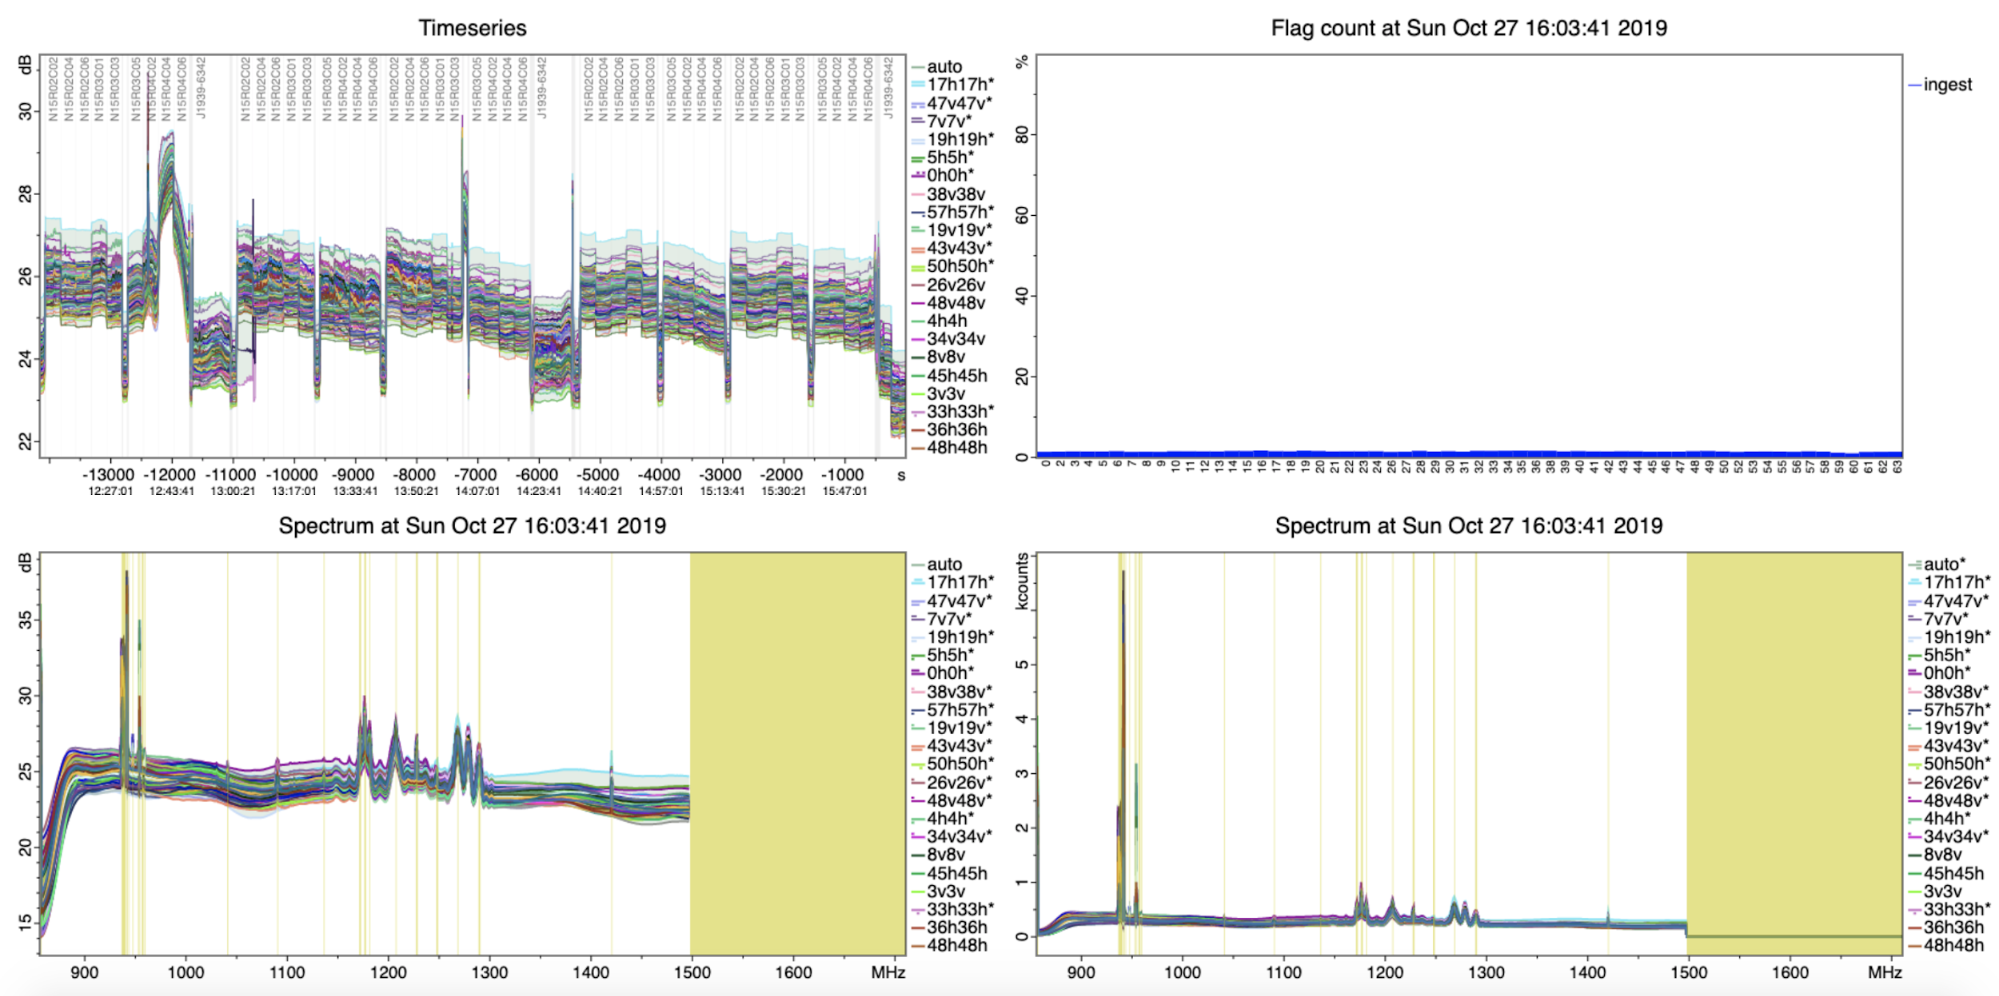
\includegraphics[scale=0.18]{Chapters/images/image65.png}
	
	%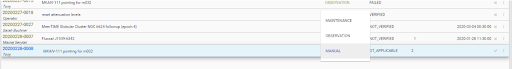
\includegraphics[resolution=100]{bur1.png}
	\caption{Part of band missing due to "no descriptors" error}
	\label{fig:image65}
\end{figure}

\begin{figure}[!thb]
	\centering
	%\includegraphicsdpi{100}{}{bur1.png}     
	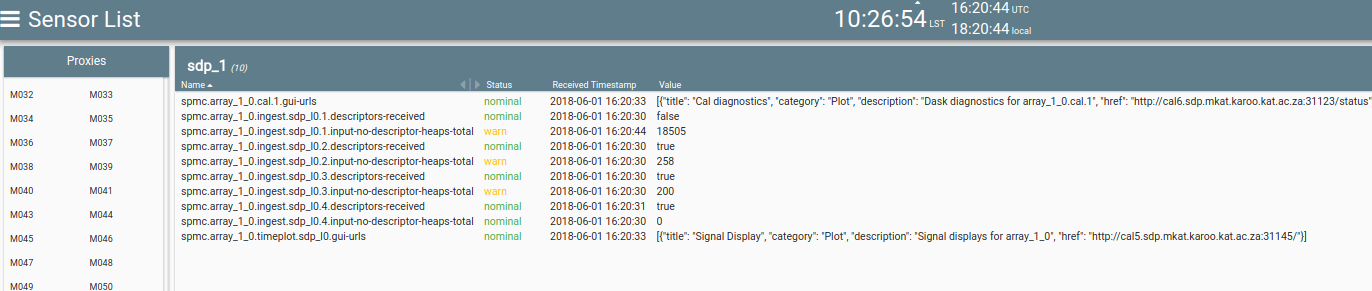
\includegraphics[scale=0.25]{Chapters/images/image37.png}
	
	%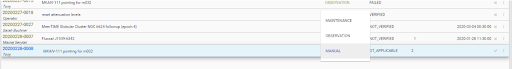
\includegraphics[resolution=100]{bur1.png}
	\caption{SDP sensor list with no-descriptor count increasing}
	\label{fig:image37}
\end{figure}



\subsection{ How to fix this}
\begin{itemize}
	\item[\textbf{Step 1}] Stop the current observation.
	  \begin{itemize}
	    \item[$\circ$] Check the number of “no descriptor” errors, check x-host health, check leaf switches, and if they are okay continue to step 2.	
    \end{itemize}

\item[\textbf{Step 2}] Tear down the array for critical/urgent observations to continue.
 \begin{itemize}
 	\item[$\circ$] This should leave the failed subarray as a zombie within SDP for debugging, while continuing operations.
 	\item[$\circ$] To diagnose if this is an SDP problem: 
 	 \begin{itemize}
	\item[$\square$] Find the time at which the ingest process stopped working: this will show up as a sudden drop in the SDP input data rate. 
	\item[$\square$] Then check SDP’s (ingest) logs for a message like this at around the same time:
	 \begin{itemize}
	 \item{} \option{2019-10-27 15:59:58.558 ing4.sdp.mkat.karoo.kat.ac.za ingest.sdp\_l0.4: array\_1\_wide\_0  worker thread blocked by full ringbuffer on heap 8467887039}	
	   \end{itemize}
    \end{itemize}	
\end{itemize}
\item[\textbf{Step 3}] After following the above steps, rebuild the subarray and monitor the leaf switches health using the following command line on obs machine : 


\begin{lstlisting}[style=DOS]
ssh kat@obs.mkat.karoo.kat.ac.za

ssh kat@obs.mkat.karoo.kat.ac.za: ./usersnfs/cbf_support/display_switch_rates.py -d leaves
\end{lstlisting}









\end{itemize}

\subsection{CBF Data Capture Failed}
See the CBF data capture error the progress out put \\
\url{http://10.97.1.13:8081/tailtask/20180612-0012/progress}
\begin{itemize}
	\item{} This error on the cbf side is caused by a clash in resources (where some skarabs are being deprogrammed in the lower cbf levels by a non lead operator)
	\item{} Break the array
\begin{lstlisting}[style=DOS]
ssh telnet cmc1.cbf.mkat.karoo.kat.ac.za 7147
?resource-list (to see which resources are available)
\end{lstlisting}

	\item{} Try building again, if this error persists over several retries contact cbf to release resources
	\item{} There is no fix in place to stop interruptions such as these - look at JIRA below
\url{https://skaafrica.atlassian.net/browse/MKAIV-1169?filter=-2}



\end{itemize}
\subsection{SDP Capture Done Failure}


 Interim SOP for CAM subarray-product-ids that end up causing sdp proxy to go in error while running scripts or rebuilding subarray.
\begin{itemize}


 	\item{} Check via the observation script logs which is visible with a warning followed by an error message.

 
	\item{} Check via CAM sensor\-list for cam data proxy, sdp\_1; filter product$-$ids value. 
\url{http://portal.mkat.karoo.kat.ac.za/katgui/sensor-list?component=sdp\_1}

If it shows more than 2 values for that same subarray, then it's a clear indication to teardown and rebuild the subarray.

Example, on subarray\_1, you will see these values: \option{array\_1\_wide\_0, array\_1\_wide\_1}

\option{Subarray-product-ids  nominal  2019-11-28 13:52:20  array\_1\_wide\_0, array\_1\_wide\_1}

\item{} Tear-down and rebuild the same subarray.  This should clear the error
\item{} Re-check via CAM sensor-list for sdp\_1; use filter: subarray-product-ids, and it should show only one value as shown in \textbf{Figure}~\ref{fig:image43}.

\option{Subarray-product-ids  nominal  2019-11-28 13:52:20 array\_1\_wide\_0}

\begin{figure}[!thb]
	\centering
	%\includegraphicsdpi{100}{}{bur1.png}     
	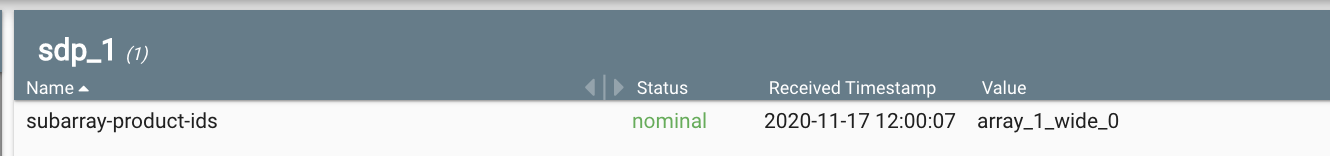
\includegraphics[scale=0.7]{Chapters/images/image43.png}
	
	%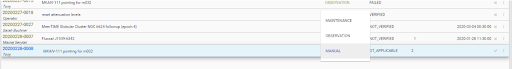
\includegraphics[resolution=100]{bur1.png}
	\caption{Subarray product-ids}
	\label{fig:image43}
\end{figure}

\textcolor{red}{Note: Only use restarting the sdp proxies via CAM as a last resort or when instructed.}
\end{itemize}

\subsection{ Vaccs Lost Sync}
When vaccs lose sync an X-engine becomes disabled
\begin{itemize}

	\item{} If during an observation, data on some band suddenly disappears as shown in . Check the signal displays as shown \textbf{Figure}~\ref{fig:image24}
	\begin{figure}[!thb]
		\centering
		%\includegraphicsdpi{100}{}{bur1.png}     
		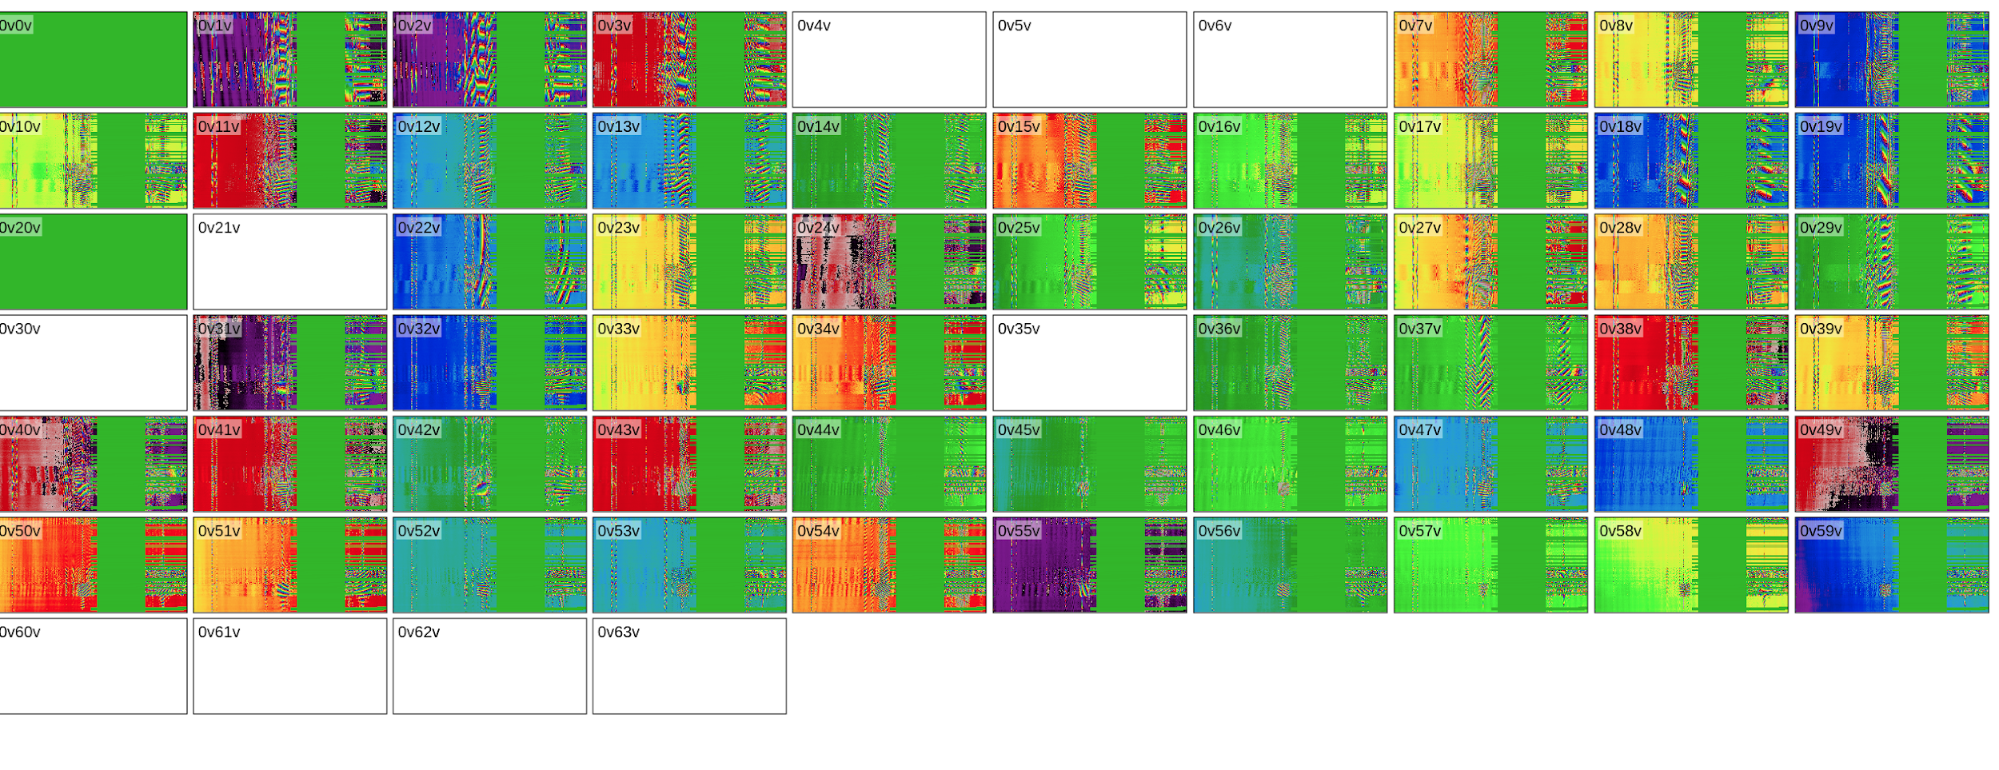
\includegraphics[scale=0.26]{Chapters/images/image24.png}
		
		%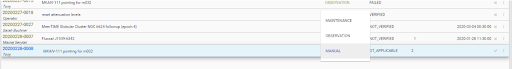
\includegraphics[resolution=100]{bur1.png}
		\caption{Data loss due to vaccs sync error}
		\label{fig:image24}
	\end{figure}

\item{} Run the check cbf health script in the obs machine
\begin{lstlisting}[style=DOS]
kat@obs.mkat.karoo.kat.ac.za:~$ ./katsdpscripts/utility/check_cbf_skarab.py  --strategy=detail
\end{lstlisting}

\item{} If the vaccs have lost sync, kill the array and build a new one
\item{} Write a JIRA with a sensorgraph as shown in \textbf{Figure}~\ref{fig:image27}



\begin{figure}[!thb]
	\centering
	%\includegraphicsdpi{100}{}{bur1.png}     
	\includegraphics[scale=0.26]{Chapters/images/image27.png}
	
	%\includegraphics[resolution=100]{bur1.png}
	\caption{CBF vaccs sync sensor graph}
	\label{fig:image27}
\end{figure}

\end{itemize}














\subsection{CBF Persistent mismatched sequence numbers}
\begin{itemize}

\item{} Apply procedure if only you are failing to build because of the errors shown in  \textbf{Figure}~\ref{fig:image95}:
\begin{figure}[!thb]
	\centering
	%\includegraphicsdpi{100}{}{bur1.png}     
	\includegraphics[scale=0.6]{Chapters/images/image95.png}
	
	%\includegraphics[resolution=100]{bur1.png}
	\caption{CBF mismatched sequence numbers error log}
	\label{fig:image95}
\end{figure}

\item{} When cbf only reports mismatched sequence errors, halt the array instrument on cmc1 and try again.  Get the array name first
\begin{lstlisting}[style=DOS]
kcpcmd -s cmc1.cbf.mkat.karoo.kat.ac.za:7147 array-list
\end{lstlisting}


\item{} Notice the highlighted instrument name in \textbf{Figure}~\ref{fig:image118} 


\begin{figure}[!thb]
	\centering
	%\includegraphicsdpi{100}{}{bur1.png}     
	\includegraphics[scale=0.6]{Chapters/images/image118.png}
	
	%\includegraphics[resolution=100]{bur1.png}
	\caption{CBF array name list}
	\label{fig:image118}
\end{figure}
\item{} Then halt the cbf instrument
\begin{lstlisting}[style=DOS]
kcpcmd -s cmc1.cbf.mkat.karoo.kat.ac.za:7147 array-halt array_name
\end{lstlisting}


\item{} Then rebuild the subarray. If you get the same error again alert the cbf team because they may need to replace the particular SKARAB board that is causing issues.
\end{itemize}

